\label{validation}

In order to ensure that the search algorithm results were valid across laser travel speeds and power levels, a range of 8 other parameters were compared with experimental results.
These experiments and simulations were the setup and analyzed as was used for the tuning experimental setup.  The base experimental parameters can be seen in Table \ref{tab:exp_constants} with the scan speed and laser power being varied as seen in Table \ref{tab:val_parameters} and the simulation material properties were used from Table \ref{tab:7000_mat_prop_complete}.
\begin{table}[!htb]
	\centering
	\caption{Validation processing parameters}
	\label{tab:val_parameters}
		\begin{tabular}{|c|c|c|} \hline 
			Exp. Id. & Scan speed (mm/min) & Laser Power (W) \\ \hline
			1 & 762 & 1000 \\ \hline  % 0
			2 & 762 & 1500 \\ \hline  % 1
			3 & 762 & 1250 \\ \hline  % 2
			4 & 1143 & 1250 \\ \hline % 3
			5 & 1143 & 1500 \\ \hline  % 5
			6 & 1524 & 1750 \\ \hline  % 6
			7 & 1524 & 1500 \\ \hline  % 7
			8 & 1524 & 2000 \\ \hline  % 8
		\end{tabular}
\end{table}
The exerimental result were collected and graphed in Figure \ref{fig:melt_track_val} and \ref{fig:melt_track_val_baseline} as the red dashed line and were used as the ground truth with which the models were compared.

These speeds and powers were first completed with the literature determined values from Table \ref{tab:starting_mat_prop_complete} and the results can be seen in Figure \ref{fig:melt_track_val_baseline}.
\begin{figure}[!htb]\centering
	\begin{subfigure}[c]{0.45\textwidth}\centering
	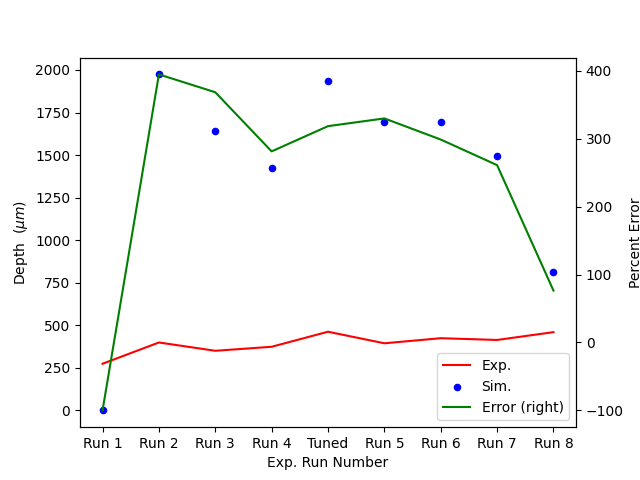
\includegraphics[width=\textwidth]{melt_track_val_baseline_depth}
	\caption{Melt track depth}
	\label{fig:melt_track_val_baseline_depth}
	\end{subfigure}\hfill{}
		\begin{subfigure}[c]{0.45\textwidth}\centering
		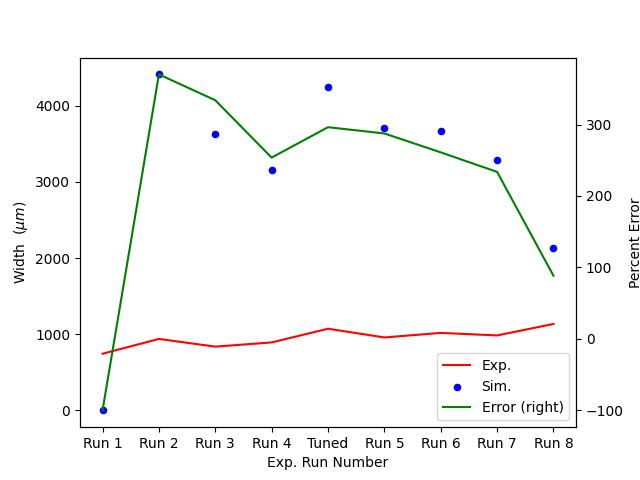
\includegraphics[width=\textwidth]{melt_track_val_baseline_width}
		\caption{Melt track width}
		\label{fig:melt_track_val_baseline_width}
		\end{subfigure}
	\caption{Comparison of experimental and simulated results for validation points with generic literature values for material dataset}
	\label{fig:melt_track_val_baseline}
\end{figure}
Where the red dashed line is the experimental results, the blue dots are the simulation predictions, and the green line is the error when comparing the simulated results to the experimental results.
These results show that over the 9 initial parameter sets, when a melt track was developed, the average absolute value of the error in the depth was approximately 290\% and the average error in the width was approximately 265\%.  To put this into terms of the response variable of the search algorithm, the sum of the width and depth error, would be 555\% combined error.
Additionally, run 1 was unable to develop a melt pool, which is contrary to the experiments where all the parameter sets had a stable melt track.  These results corroborate the results from Figure \ref{fig:response_complete} which showed that the parameter set used for tuning initial dataset of material properties found in the literature is wholly inadequate for simulating the process at hand. 

In contrast to these results, the material dataset which was found in Table \ref{tab:7000_mat_prop_complete} was used to simulate each parameter set, and the results can be seen in Figure \ref{fig:melt_track_val}.
\begin{figure}[!htb]\centering
	\begin{subfigure}[c]{0.45\textwidth}\centering
	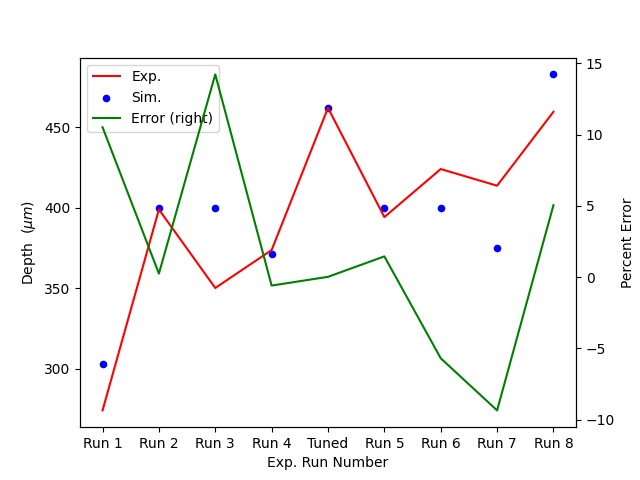
\includegraphics[width=\textwidth]{melt_track_val_depth}
	\caption{Melt track depth}
	\label{fig:melt_track_val_depth}
	\end{subfigure}\hfill{}
		\begin{subfigure}[c]{0.45\textwidth}\centering
		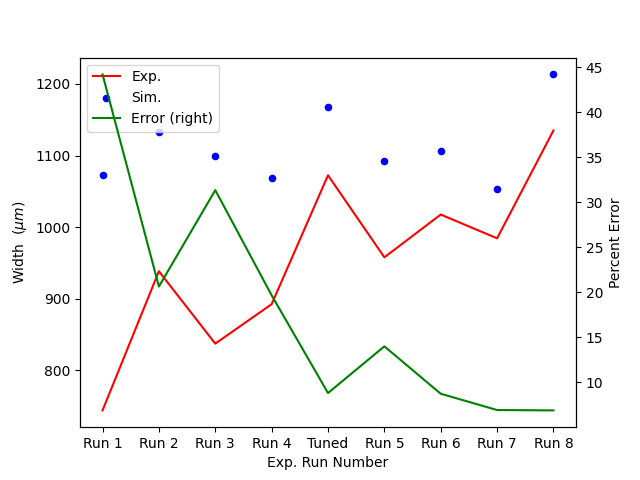
\includegraphics[width=\textwidth]{melt_track_val_width}
		\caption{Melt track width}
		\label{fig:melt_track_val_width}
		\end{subfigure}
	\caption{Comparison of experimental and simulated results for validation points with optimized values for material dataset}
	\label{fig:melt_track_val}
\end{figure}
Where the red dashed line is the experimental results, the blue dots are the simulation predictions, and the green line is the error when comparing the simulated results to the experimental results.
These results show the average error in the width was approximately 17\% and the average error in the depth was approximately 5\%, which creates a combined error of only 22\%.  These results show that the optimized dataset is better at predicting the combined error of the simulation by over 500\%.  This results in a simulation which can be leveraged more intensely during the process development and build qualification process.  
These results are from a wide parameter set which encompasses most of the usable parameter space for deposition found experimentally.  This improvement in accuracy will allow for a greater application in the model in the determination of an optimized parameter set for a given build.  In addition, the model is seen to be more accurate at parameters above the parameter used during the optimization.  This leads to the conclusion that if a more accurate simulation is needed, the optimization should be done at a parameter set near the desired parameter set.